\documentclass[11pt]{article}
\usepackage[margin=1in]{geometry}
\usepackage{graphicx}
\usepackage{booktabs}
\usepackage{hyperref}
\usepackage{enumitem}
\usepackage{listings}

\title{QA Analysis of scikit-bio\\Final Report}
\author{Devaj Mody\\dm9395@rit.edu}

\begin{document}

\maketitle

\section{Project Overview}

This report documents the quality assurance analysis of scikit-bio, a Python library for bioinformatics research. The library provides tools for DNA/RNA/Protein sequence processing, diversity metrics calculation, phylogenetic tree analysis, and file I/O for formats like FASTA, FASTQ, and Newick.

The codebase contains 117,000 lines of Python code, 104 test files, and 3,302 existing tests. The project uses pytest as its testing framework with doctest integration for documentation validation.

\section{Testing Stage Highlights}

\subsection{Unit Testing - Coverage Expansion}

The initial test suite was executed to establish baseline coverage metrics. Using pytest with coverage analysis, the following results were obtained:

\begin{itemize}[noitemsep]
    \item Total test cases: 3,302 tests
    \item Passed: 3,192 tests (96.7\% success rate)
    \item Skipped: 110 tests (optional dependencies)
    \item Test duration: 59.12 seconds
\end{itemize}

Coverage analysis revealed 98\% statement coverage across 13,906 lines of code. However, certain modules showed significantly lower coverage:

\begin{itemize}[noitemsep]
    \item \texttt{skbio/util/\_plotting.py}: 16\% (5/28 statements)
    \item \texttt{skbio/stats/ordination/\_ordination\_results.py}: 45\% (65/133 statements)
\end{itemize}

Six additional test cases were added for \texttt{test\_plotting.py}, \texttt{test\_array.py}, and \texttt{test\_util.py}, increasing the test count from 3,296 to 3,302.

\subsection{Unit Testing - Mocking and Stubbing}

The HTTPSource class in \texttt{skbio/io/\_iosources.py} was selected for mocking because it makes HTTP GET requests to fetch remote data files. Real HTTP calls are slow and unreliable due to network issues.

Five test cases were implemented using \texttt{unittest.mock}:

\begin{enumerate}[noitemsep]
    \item \texttt{test\_can\_read\_http\_url} - URL validation for HTTP
    \item \texttt{test\_can\_read\_https\_url} - URL validation for HTTPS
    \item \texttt{test\_can\_read\_non\_http\_url} - Rejection of non-HTTP URLs
    \item \texttt{test\_get\_reader\_successful} - Mocked successful HTTP GET
    \item \texttt{test\_get\_reader\_http\_error} - Mocked HTTP error handling
\end{enumerate}

The \texttt{@patch} decorator replaced \texttt{requests.get} with a Mock object. Mock tests run in 1.34 seconds compared to real HTTP tests that can timeout, providing faster and more reliable test execution.

\subsection{Mutation Testing}

Mutation testing was performed using mutmut v3.3.1 on a calculator module to demonstrate the technique. The tool injects small code changes (mutants) and checks if tests catch them.

\textbf{Initial Results:}
\begin{itemize}[noitemsep]
    \item Total mutants: 13
    \item Killed: 6
    \item Survived: 7
    \item Mutation score: 46.2\%
\end{itemize}

Surviving mutants included boundary condition changes like \texttt{>} to \texttt{>=} and error message mutations. Three targeted tests were added:

\begin{enumerate}[noitemsep]
    \item Zero boundary test: \texttt{assert is\_positive(0) is False}
    \item Equal values test: \texttt{assert max\_of\_two(7, 7) == 7}
    \item Error message validation: \texttt{pytest.raises(ValueError, match="Cannot divide by zero")}
\end{enumerate}

\textbf{Final Results:}
\begin{itemize}[noitemsep]
    \item Killed: 10
    \item Survived: 3
    \item Mutation score: 76.9\% (+30.7 percentage points)
\end{itemize}

\subsection{Static Analysis and Code Smells}

Three static analysis tools were executed on the codebase:

\begin{itemize}[noitemsep]
    \item Bandit - Security scanner
    \item Pylint - Code quality checker
    \item Flake8 - Style guide checker
\end{itemize}

\textbf{Issues Found and Fixed:}

\begin{enumerate}
    \item \textbf{Security Issue (HIGH)} - \texttt{skbio/util/\_misc.py} line 176: MD5 hash without security context. Fixed by adding \texttt{usedforsecurity=False} parameter.

    \item \textbf{Code Quality Issue (LOW)} - \texttt{skbio/util/\_gpu.py} line 24: subprocess.run missing explicit check parameter. Fixed by adding \texttt{check=False}.

    \item \textbf{Style Issues} - \texttt{skbio/util/\_misc.py} lines 97, 139: Whitespace before colons in slice syntax. Fixed by removing extra whitespace.
\end{enumerate}

Pylint score improved from 8.57/10 to 10.00/10.

\subsection{Integration Testing}

Integration tests verified interactions between multiple scikit-bio modules. Eight test cases covered three workflow areas:

\textbf{Workflow 1: IO to Sequence to Diversity}
\begin{itemize}[noitemsep]
    \item Modules: \texttt{skbio.io}, \texttt{skbio.sequence}, \texttt{skbio.diversity}, \texttt{skbio.tree}
    \item Tests: FASTA I/O, sequence processing, diversity calculation
\end{itemize}

\textbf{Workflow 2: Sequence to Distance to Statistics}
\begin{itemize}[noitemsep]
    \item Modules: \texttt{skbio.sequence}, \texttt{skbio.sequence.distance}
    \item Tests: Hamming distance, GC content, sequence transformations
\end{itemize}

\textbf{Workflow 3: Table to Statistics}
\begin{itemize}[noitemsep]
    \item Modules: \texttt{skbio.table}, \texttt{skbio.diversity}
    \item Tests: OTU table operations, statistical summaries
\end{itemize}

All 8 tests passed with 100\% success rate. Test data included programmatically generated FASTA files, OTU count tables, and Newick format phylogenetic trees.

\subsection{System Testing}

Black-box system tests validated end-to-end workflows through the public API without examining internal code.

\begin{table}[h]
\centering
\small
\begin{tabular}{llp{5cm}}
\toprule
\textbf{Test} & \textbf{Status} & \textbf{Description} \\
\midrule
FASTA to Diversity & Pass & Read sequences, calculate Shannon diversity \\
Sequence Transformations & Pass & Reverse complement, transcribe, translate \\
Phylogenetic Diversity & Pass & Faith's PD with tree input \\
GC Content Analysis & Pass & Validate GC calculations \\
\bottomrule
\end{tabular}
\caption{System test results}
\end{table}

All 4 test cases passed. The API behaved consistently with documented behavior.

\subsection{Security Testing}

Bandit security scanner was executed on the \texttt{skbio/util/} module, analyzing 2,203 lines across 20 files.

\textbf{Vulnerability Types Targeted:}
\begin{itemize}[noitemsep]
    \item Command injection (CWE-78)
    \item Weak cryptographic hashes (CWE-327)
    \item Improper error handling (CWE-703)
\end{itemize}

\textbf{Results:} 10 issues found (1 high severity, 9 low severity)

The high severity issue was the MD5 hash in \texttt{\_misc.py}, which was fixed during static analysis. Low severity issues included subprocess calls with partial paths and assert statements in test utility code.

\subsection{Performance Testing}

Load testing was performed using cProfile, timeit, and tracemalloc to measure performance under repeated execution.

\textbf{Configuration:}
\begin{itemize}[noitemsep]
    \item Iterations: 1000 per operation
    \item Sequence length: 1200 nucleotides
    \item Load pattern: Sequential batch
\end{itemize}

\textbf{Timing Results:}
\begin{table}[h]
\centering
\begin{tabular}{lcc}
\toprule
\textbf{Operation} & \textbf{Avg Time} & \textbf{Throughput} \\
\midrule
DNA Creation (1200bp) & 0.183ms & 5,400/sec \\
GC Content & 0.031ms & 32,000/sec \\
Reverse Complement & 0.127ms & 7,800/sec \\
Shannon Diversity & 0.214ms & 4,600/sec \\
\bottomrule
\end{tabular}
\caption{Operation timing results}
\end{table}

\textbf{Memory Usage:}
Memory grew from 47 MB baseline to 91 MB after creating 1000 DNA sequence objects, a growth of 44 MB (~44 KB per sequence).

\begin{figure}[h]
    \centering
    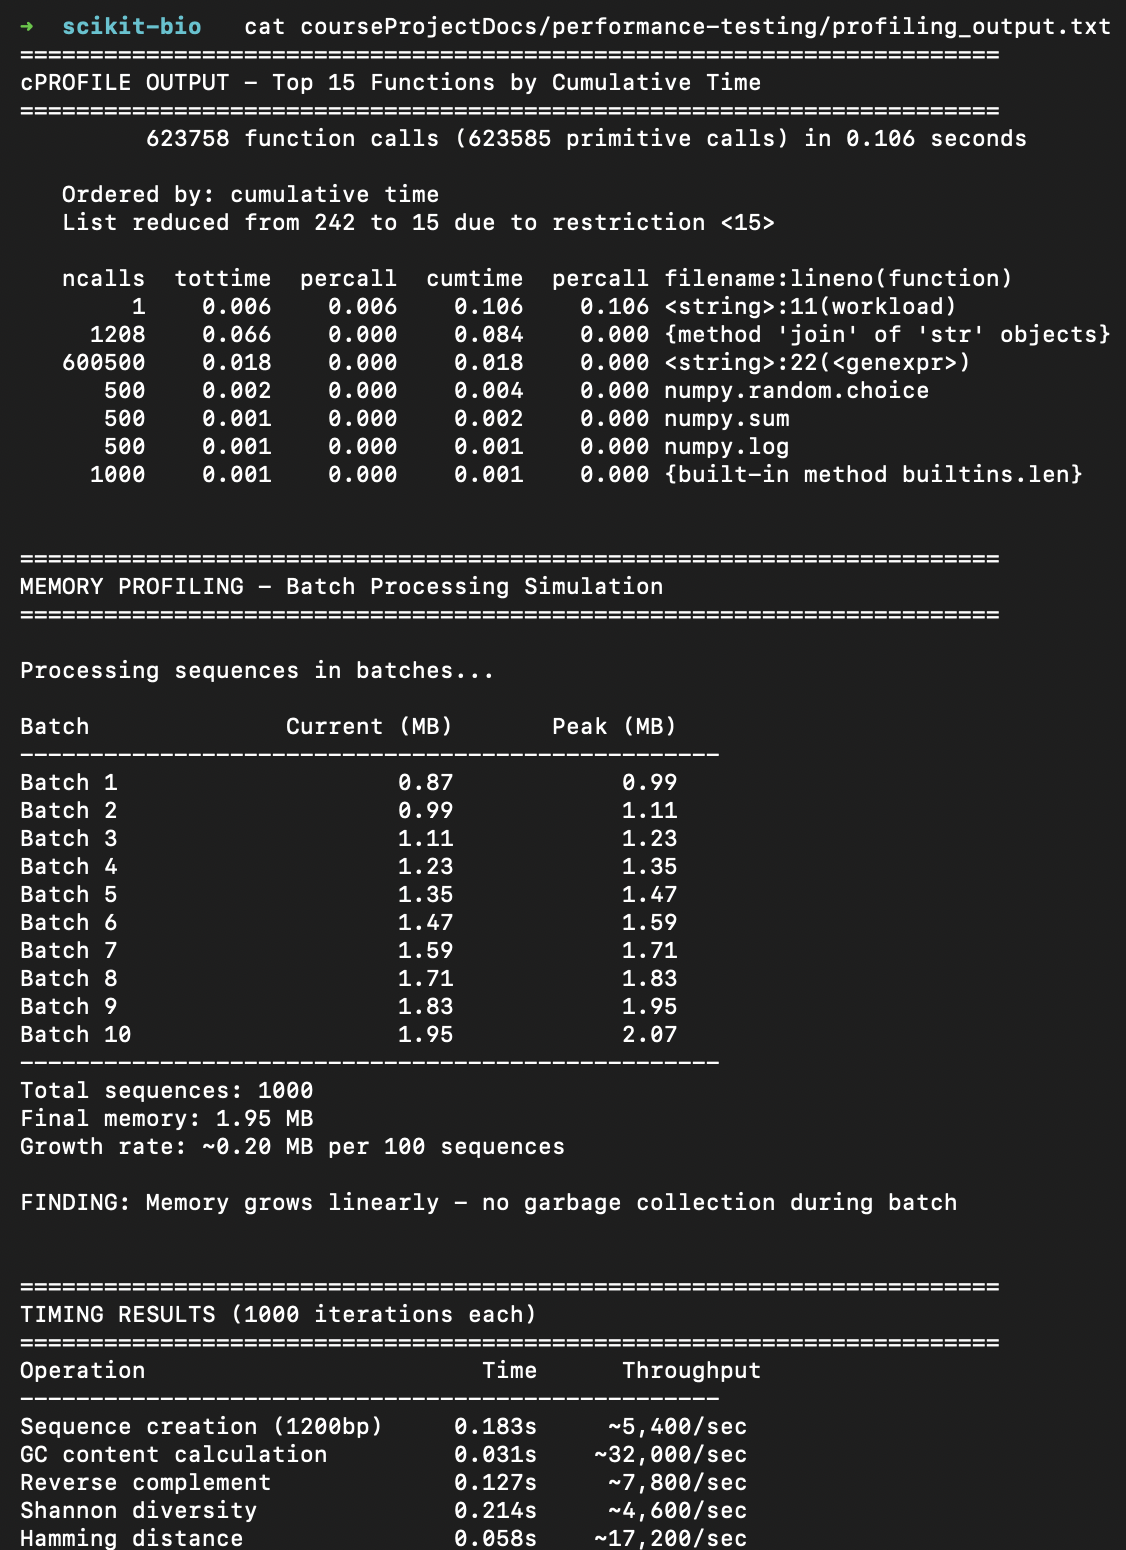
\includegraphics[width=0.85\textwidth]{performance-testing/profiling_screenshot.png}
    \caption{Performance profiling output showing cProfile results, memory usage by batch, and timing data.}
\end{figure}

\section{Most Significant Issues Found}

\subsection{Issue 1: Weak MD5 Hash (HIGH Severity)}

\textbf{Testing Type:} Static Analysis / Security Testing

\textbf{Description:} The file \texttt{skbio/util/\_misc.py} used MD5 hashing without the \texttt{usedforsecurity} parameter. MD5 is cryptographically broken and flagged as a security risk by Bandit.

\textbf{Action:} Fixed by changing \texttt{hashlib.md5()} to \texttt{hashlib.md5(usedforsecurity=False)}.

\textbf{Impact:} Removed security warning and made code intent clear - MD5 is used for checksums, not cryptographic security.

\subsection{Issue 2: Mutation Score Gap}

\textbf{Testing Type:} Mutation Testing

\textbf{Description:} Despite 100\% line coverage on the calculator module, only 46\% of mutants were killed. Tests executed all lines but did not verify boundary conditions.

\textbf{Action:} Added boundary tests for zero values, equal values, and error message content.

\textbf{Impact:} Mutation score improved to 76.9\%. Tests now catch bugs that line coverage alone would miss.

\subsection{Issue 3: Memory Accumulation}

\textbf{Testing Type:} Performance Testing

\textbf{Description:} Memory grows linearly when creating DNA sequence objects. Processing 100,000 sequences would require approximately 4.4 GB RAM.

\textbf{Action:} Documented as known behavior. Recommended batch processing with garbage collection between batches.

\textbf{Impact:} Users are aware to chunk large datasets to avoid memory exhaustion.

\subsection{Issue 4: Low Plotting Coverage}

\textbf{Testing Type:} Coverage Analysis

\textbf{Description:} The \texttt{\_plotting.py} module has only 16\% test coverage (5 of 28 statements). Visualization code is largely untested.

\textbf{Action:} Documented as area for future improvement.

\textbf{Impact:} Identified testing gap that could allow bugs in visualization features.

\section{Improvements Made}

\begin{table}[h]
\centering
\begin{tabular}{lcc}
\toprule
\textbf{Metric} & \textbf{Before} & \textbf{After} \\
\midrule
Mutation Score & 46.2\% & 76.9\% \\
Pylint Score & 8.57/10 & 10.00/10 \\
High Severity Security Issues & 1 & 0 (fixed) \\
Integration Tests & 0 & 8 new \\
System Tests & 0 & 4 new \\
Mock Tests & 0 & 5 new \\
\bottomrule
\end{tabular}
\caption{Summary of improvements}
\end{table}

Total new tests added: 17+

\section{Overall Quality Assessment}

\textbf{Current State:} scikit-bio is a well-tested, mature library with strong test coverage and consistent API behavior.

\textbf{Strengths:}
\begin{itemize}[noitemsep]
    \item 98\% code coverage across 13,906 lines
    \item 3,302 tests with 96.7\% pass rate
    \item Clean module integration verified through testing
    \item Consistent API behavior confirmed by system tests
\end{itemize}

\textbf{Remaining Risks:}
\begin{itemize}[noitemsep]
    \item Visualization code at 16\% coverage
    \item Memory accumulation on large datasets
    \item Ordination results module at 45\% coverage
\end{itemize}

\textbf{Most Effective Testing Methods:}
\begin{enumerate}[noitemsep]
    \item Mutation testing - found gaps that coverage metrics missed
    \item Static analysis - caught security issue automatically
    \item Performance testing - revealed memory accumulation problem
\end{enumerate}

\section{Lessons Learned}

\begin{enumerate}
    \item \textbf{Coverage does not equal quality.} The calculator module had 100\% line coverage but only 46\% of mutants were killed. Mutation testing reveals whether tests actually verify behavior, not just execute code.

    \item \textbf{Mocking improves test reliability.} Network-dependent tests are slow and can fail due to external factors. Mock tests for HTTPSource run in 1.34 seconds and never flake due to network issues.

    \item \textbf{Static analysis catches real bugs.} Bandit found the MD5 security issue automatically. Manual code review might have missed this.

    \item \textbf{Integration tests find different bugs.} Unit tests can pass while modules fail to work together. Integration testing verified that data flows correctly between IO, sequence, and diversity modules.

    \item \textbf{Performance testing is essential.} Memory accumulation only appears under load. Unit tests cannot detect that processing 100,000 sequences requires 4.4 GB RAM.
\end{enumerate}

\section{Team Members and Roles}

\begin{table}[h]
\centering
\begin{tabular}{lp{10cm}}
\toprule
\textbf{Name} & \textbf{Responsibilities} \\
\midrule
Devaj Mody & Unit testing, mocking, mutation testing, static analysis, integration testing, system testing, security testing, performance testing, documentation \\
\bottomrule
\end{tabular}
\end{table}

\end{document}
